\documentclass[9pt]{beamer}
\mode<presentation>
\usepackage[T1]{fontenc}
\usepackage{color}
\usepackage{graphicx}
\usepackage{natbib}
\usepackage{tikz}
\usetikzlibrary{shapes.geometric}
\usepackage{xmpmulti}
\usepackage{animate}
\usepackage{tcolorbox}
\usepackage{amsmath}
\usepackage{gensymb}
\usepackage{adjustbox}
\usepackage{todonotes}
%\usepackage{polyglossia}
\usepackage{textgreek}

\usetheme{Boadilla}
%\usecolortheme{seahorse}

\usefonttheme{professionalfonts}

\title[A Topography of Climate Research]{A Topography of Climate Change Research}
\author{Max Callaghan }
\institute[MCC]{
	\url{callaghan[at]mcc-berlin.net} \\
	
\includegraphics[height=1cm,width=2cm]{MCC_Logo_RZ_rgb.jpg} \\ \medskip Mercator Research on Global Commons and Climate Change \\ School of Earth and Environment, University of Leeds
}


\newtheorem*{remark}{}

\bibliographystyle{apalike}

\begin{document}
	
\begin{frame}
	\titlepage
\end{frame}



\begin{frame}{Introduction}
	\begin{columns}
		\begin{column}{0.6\linewidth}
			\begin{center}
				\begin{figure}
					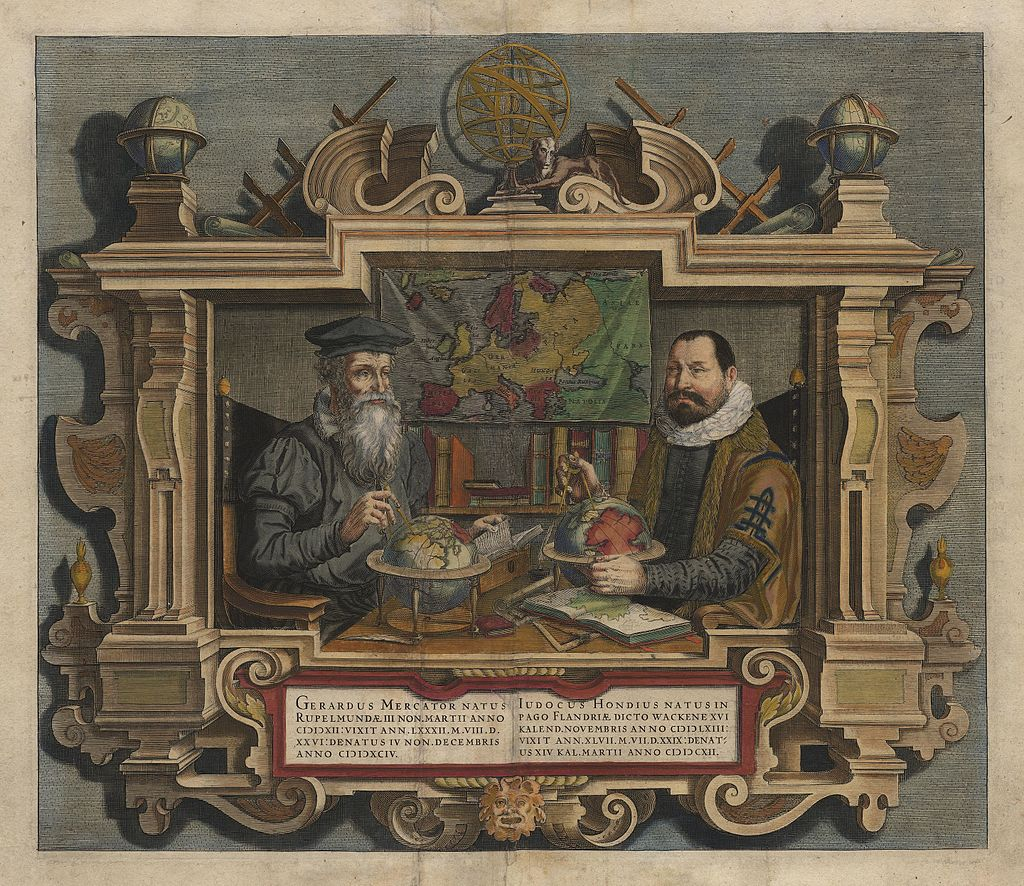
\includegraphics[width=1\linewidth]{../plots/Hondius_Portrait_of_map-makers}
					\caption{Portrait of map-makers, Gerard Mercator and Jodocus Hondius (Jodocus Hondius) source: Wikipedia Commons}
				\end{figure}
			\end{center}
		\end{column}
		\begin{column}{0.4\linewidth}
			\begin{center}
				\begin{itemize}
					\item<2-> Topography is a description of a landscape
					\item<3-> Topics (from the Greek \texttau\textomikron\textpi\textomikron\textvarsigma, place) can describe the features of a body of text
				\end{itemize}
			\end{center}
		\end{column}
	\end{columns}
\end{frame}

\begin{frame}{Outline}

\tableofcontents

\end{frame}

\section{Motivation}

\begin{frame}{Literature growth}

\begin{columns}
	\begin{column}{0.618\linewidth}
		\begin{figure}
			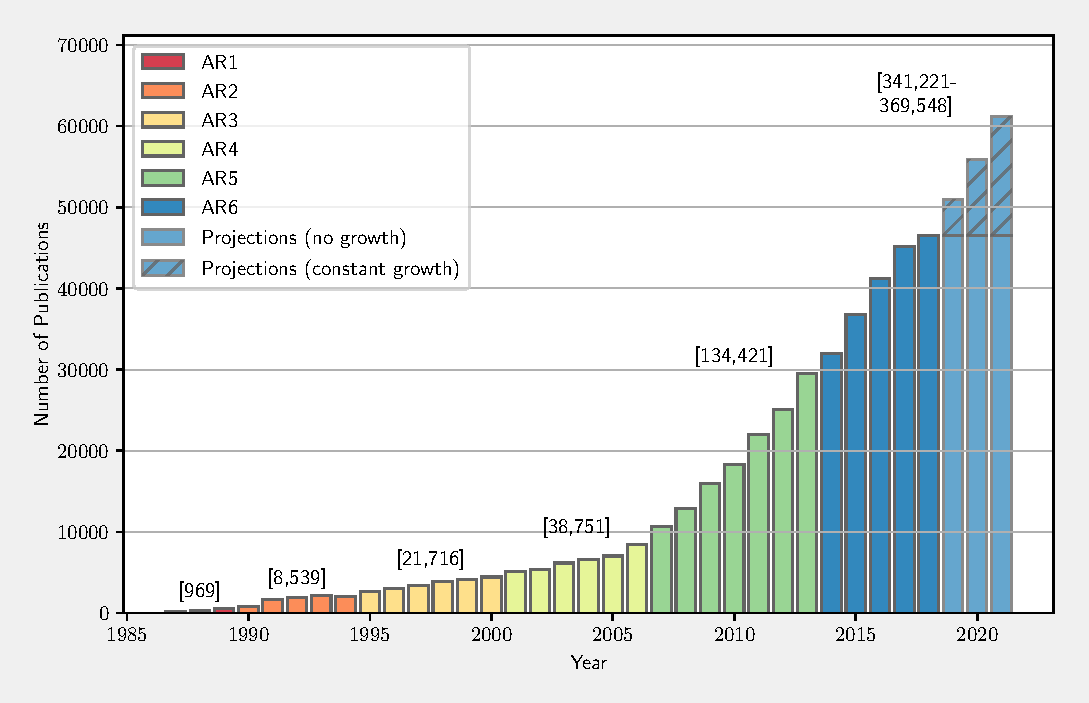
\includegraphics[width=\linewidth]{../plots/literature_size/pubs_time.pdf}
			\caption{Updated from \citet{Minx2017l}}
		\end{figure}
	\end{column}
	\begin{column}{0.382\linewidth}
		\begin{itemize}
			\item<2->  The Literature on climate change has grown, and continues to grow
			\item<3-> A general understanding of the literature becomes ever more difficult
			
		\end{itemize}
	\end{column}
\end{columns}

\end{frame}

\begin{frame}{Literature growth}

\begin{columns}
	\begin{column}{0.382\linewidth}
	\begin{itemize}
		\item<1->We entrust the IPCC with providing a \textit{comprehensive} and \textit{transparent} assessment of the literature 
		\item<2->Although IPCC reports cite ever greater numbers of papers, this number decreases in proportion to the number of papers in literature
		
	\end{itemize}
\end{column}
	\begin{column}{0.618\linewidth}<2->
		\begin{figure}
			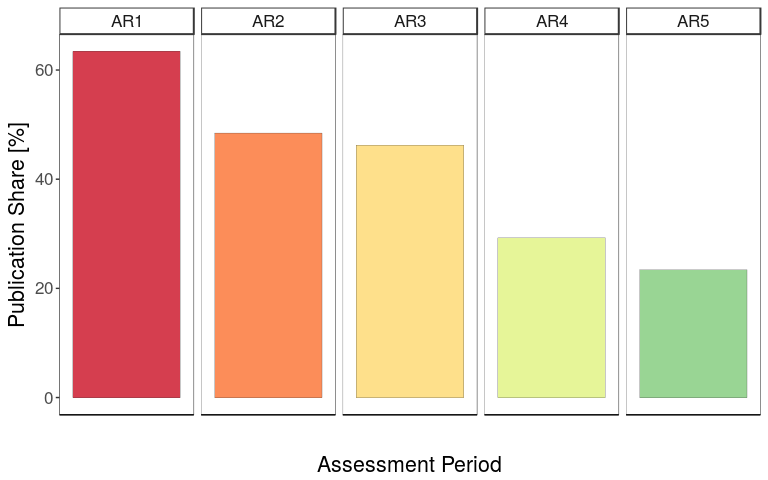
\includegraphics[width=\linewidth]{../plots/wos_IPCC_shares.png}
			\caption{\citep{Minx2017l}}
		\end{figure}
	\end{column}
\end{columns}

\end{frame}

\begin{frame}{Research Questions}
\begin{itemize}
	\item<1-> What is the literature about?
	\item<2-> Does the IPCC cite some areas of the literature more than others?
\end{itemize}
\end{frame}

\section{Approach}

\begin{frame}{Data - Words, words, words}
	
	\begin{table}[h]
		\begin{adjustbox}{width=\linewidth}
			\begin{tabular}{|l |p{1.8cm} p{1.8cm} p{1.8cm} p{1.8cm} p{1.8cm} p{1.8cm}|} 
\hline 
&\textbf{AR1} & \textbf{AR2} & \textbf{AR3} & \textbf{AR4} & \textbf{AR5} & \textbf{AR6}\\ \hline\textbf{Years} &1986-1989 & 1990-1994 & 1995-2000 & 2001-2006 & 2007-2013 & 2014-\\ 
\textbf{Documents} &1,167 & 8,539 & 21,716 & 38,750 & 134,413 & 201,606\\ 
\textbf{Unique words} &2,000 & 12,480 & 23,346 & 34,637 & 71,867 & 94,746\\ 
\textbf{New words} & change (560) & oil (287) & downscaling (217) & sres (234) & biochar (1,791) & mmms (313)\\ & climate (428) & deltac (283) & degreesc (187) & petm (95) & redd (1,113) & cop21 (234)\\ & co2 (318) & whole (256) & ncep (130) & amf (88) & cmip5 (679) & c3n4 (214)\\ & climatic (289) & tax (254) & fco (107) & sf5cf3 (86) & cmip3 (587) & sdg (187)\\ & model (288) & landscape (249) & pfc (98) & clc (81) & mofs (299) & zika (182)\\ & atmospheric (281) & alternative (243) & otcs (98) & embankment (81) & sdm (297) & ndcs (168)\\ & effect (280) & availability (242) & dtr (95) & cwd (79) & mof (275) & indc (164)\\ & global (224) & life (239) & nee (89) & etm (75) & biochars (252) & indcs (134) \\ \hline
\end{tabular}

		\end{adjustbox}			
		\caption{Growth in climate change literature}
		\label{growthtable}
	\end{table}	

%		\begin{itemize}
%			\item bla
%			
%		\end{itemize}

Data from WoS Core Collection, query following \citet{Grieneisen2011}

\end{frame}

\begin{frame}{Approach - What is the matter?}

\begin{columns}
	\begin{column}{0.382\linewidth}
		\begin{itemize}
			\item<1-> Topic modelling \citep{Blei2012} describes a suite of algorithms to discover the latent semantic content of documents
			\item<2-> NMF \citep{Lee1999} is a dimensionality reduction technique that can be used for topic modelling
			\item<3-> I follow \citet{Greene2016} in using NMF to generate static models of time windows (ARs 1-6) and a topic model of these topic models to generate dynamic topics, which describe topics across time 
			
		\end{itemize}
	\end{column}
	\begin{column}{0.618\linewidth}<2->
		\only<2->{\(V_{i\mu} \) is a term frequency-inverse document frequency matrix of \textit{stemmed} terms} 
		\only<2->{\[V_{i\mu} \approx (WH)_{i\mu} = \sum_{a=1}^{r}W_{ia}H_{a\mu} \] \(V\) is approximated by the product of \(W\) and \(H\)}
		
		\begin{figure}
			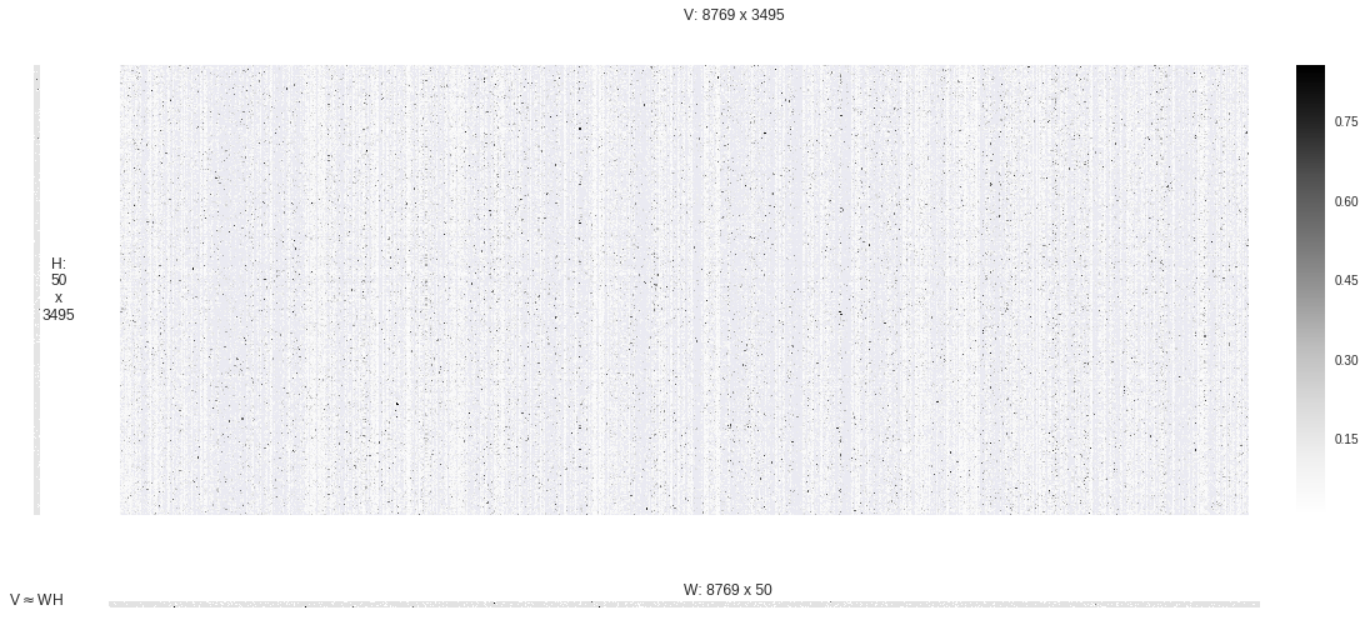
\includegraphics[width=\linewidth]{../plots/VWH.png}
		\end{figure}
	\end{column}

\end{columns}

\end{frame}

\section{Results}

%%%%%%%%%%%%%%%%%%%%%%%%%%%%%%%%%%

\begin{frame}{Topics and Disciplines}
\begin{columns}
	\begin{column}{0.618\linewidth}
		\begin{figure}
			\begin{center}
				%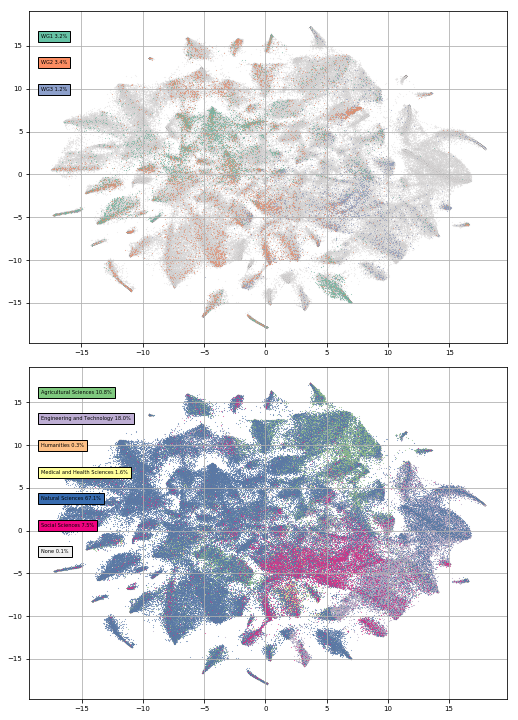
\includegraphics[width=1\linewidth]{tsne_results/plots/run_665_s_0_p200_double.pdf}
				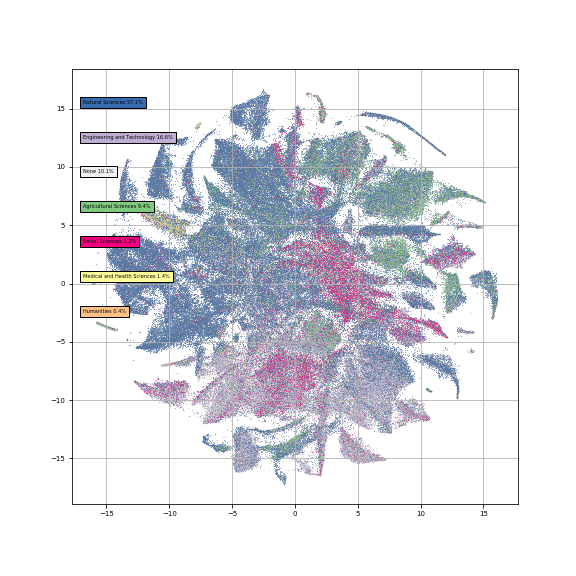
\includegraphics[width=0.8\linewidth]{../tsne_results/plots/run_1429_s_0_p50_oecds.png}
				\caption{A map of the literature on climate change. Document positions are obtained by reducing the topic scores to two dimensions via t-SNE Documents are coloured by web of science discipline category. See SI table for topic composition of each grid square}
				\label{map-oecd}
			\end{center}
		\end{figure}
	\end{column}
	\begin{column}{0.382\linewidth}
		\begin{itemize}
			\item<2-> Corpus mainly natural sciences
			\item<3-> Topic space maps to disciplinary structure, with cross-cutting topic areas, e.g. social science and engineering
			
		\end{itemize}
	\end{column}
\end{columns}
\end{frame}

%%%%%%%%%%%%%%%%%%%%%%%%%%%%%%%

%\begin{frame}{Topics and Disciplines}
%\begin{columns}
%	\begin{column}{0.618\linewidth}
%		\begin{figure}
%			\includegraphics[width=\linewidth]{example-image}
%		\end{figure}
%	\end{column}
%	\begin{column}{0.382\linewidth}
%		\begin{itemize}
%			\item TODO: map topics to categories		
%		\end{itemize}
%	\end{column}
%\end{columns}
%\end{frame}

%%%%%%%%%%%%%%%%%%%%%%%%%%%%%%%

\begin{frame}{Disciplinary representation}
\begin{columns}
	\begin{column}{0.382\linewidth}
	\begin{itemize}
		\item<1-> The social sciences are seen as under-represented in IPCC reports
		\item<3-> \citet{Bjurström2011} even name biases in IPCC citation patterns
		\item<4-> These statements are based on observed disciplinary makeup of IPCC citations
		
	\end{itemize}
\end{column}
	\begin{column}{0.618\linewidth}<2->
		\begin{figure}[h!]
			\begin{center}
				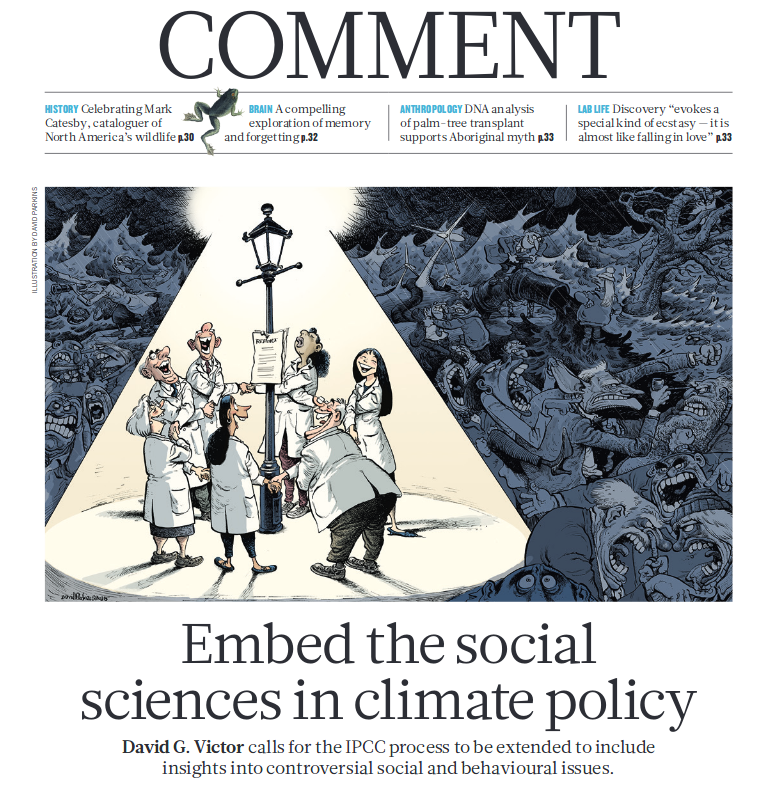
\includegraphics[width=0.85\linewidth]{../plots/victor.png}
				\caption{\citep{Victor2015}}
			\end{center}
		\end{figure}
	\end{column}
\end{columns}
\end{frame}

%%%%%%%%%%%%%%%%%%%%%%%%%%%%%%%%%%

\begin{frame}{Disciplinary representation}
\begin{columns}
	\begin{column}{0.618\linewidth}
\begin{figure}[h!]
	\begin{center}
		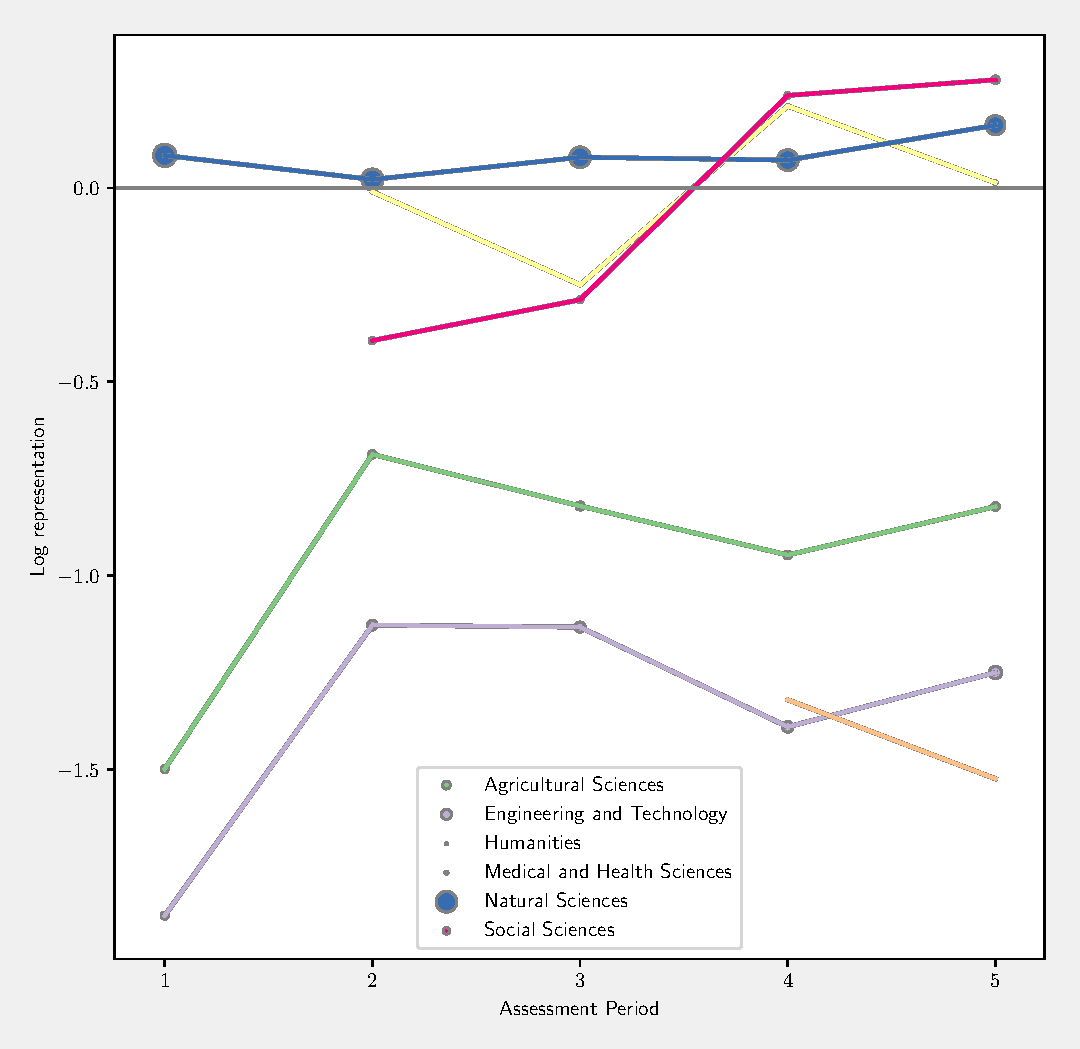
\includegraphics[width=0.85\linewidth]{../plots/ipcc_representation/ipcc_rep_oecds_time.pdf}
		\caption{The representation within the IPCC of each discipline over time}
		\label{oecd_rep}
	\end{center}
\end{figure}
	\end{column}
	\begin{column}{0.382\linewidth}
		\begin{itemize}
			\item<1-> Natural sciences have remained a large part of the literature and well-represented in IPCC reports. 
			\item<2-> The social sciences have long been over-represented
			\item<3-> Agricultural sciences and engineering are the most clearly under-represented (humanities make up a very small portion of the literature)
			
		\end{itemize}
	\end{column}
\end{columns}
\end{frame}

%%%%%%%%%%%%%%%%%%%%%%%%%%%%%%%%%%

\begin{frame}{The Social Sciences}
\begin{columns}
	\begin{column}{0.618\linewidth}
		\begin{figure}
			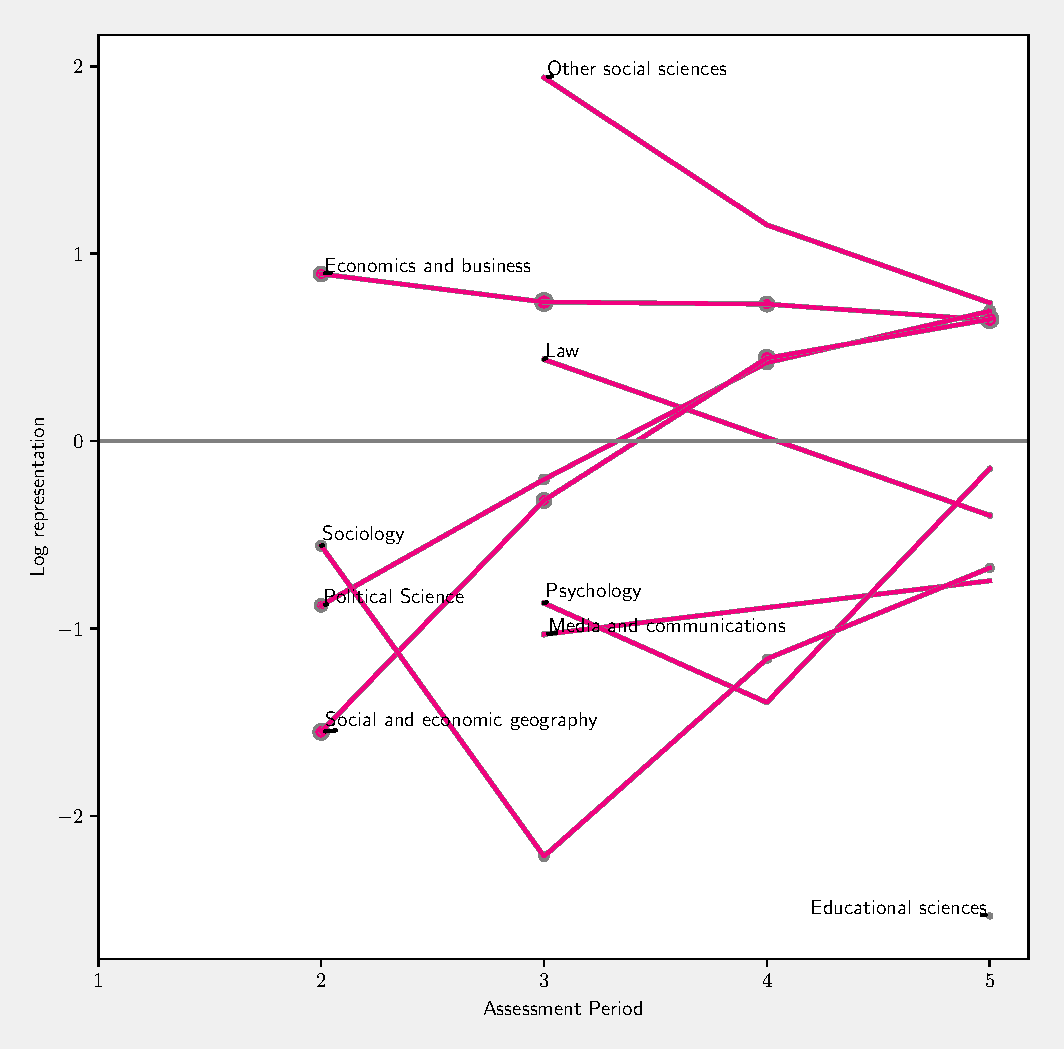
\includegraphics[width=\linewidth]{../plots/ipcc_representation/ipcc_rep_cats_time_Social_Sciences.pdf}
		\end{figure}
	\end{column}
	\begin{column}{0.382\linewidth}
		\begin{itemize}
			\item<1->  Economics has remained over-represented
			\item<2-> Political science and social and economic geography large under-represented literatures that have now become over-represented
			\item<3-> Sociology and Psychology remain small parts of the literature that are also under-represented
			
		\end{itemize}
	\end{column}
\end{columns}
\end{frame}

%%%%%%%%%%%%%%%%%%%%%%%%%%%%%%%%%%

\begin{frame}{IPCC Working Groups}
\begin{columns}
	\begin{column}{0.618\linewidth}
		\begin{figure}
		\only{
	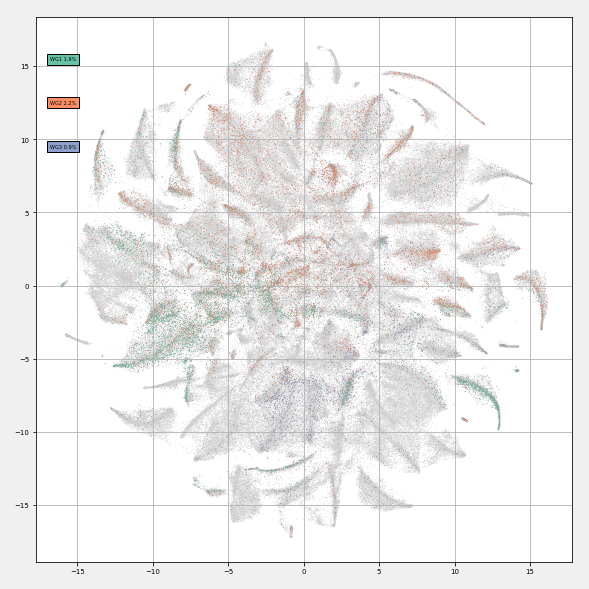
\includegraphics[width=0.8\linewidth]{../tsne_results/plots/run_1429_s_0_p50_wgs.png}
}<1>
		\only{
		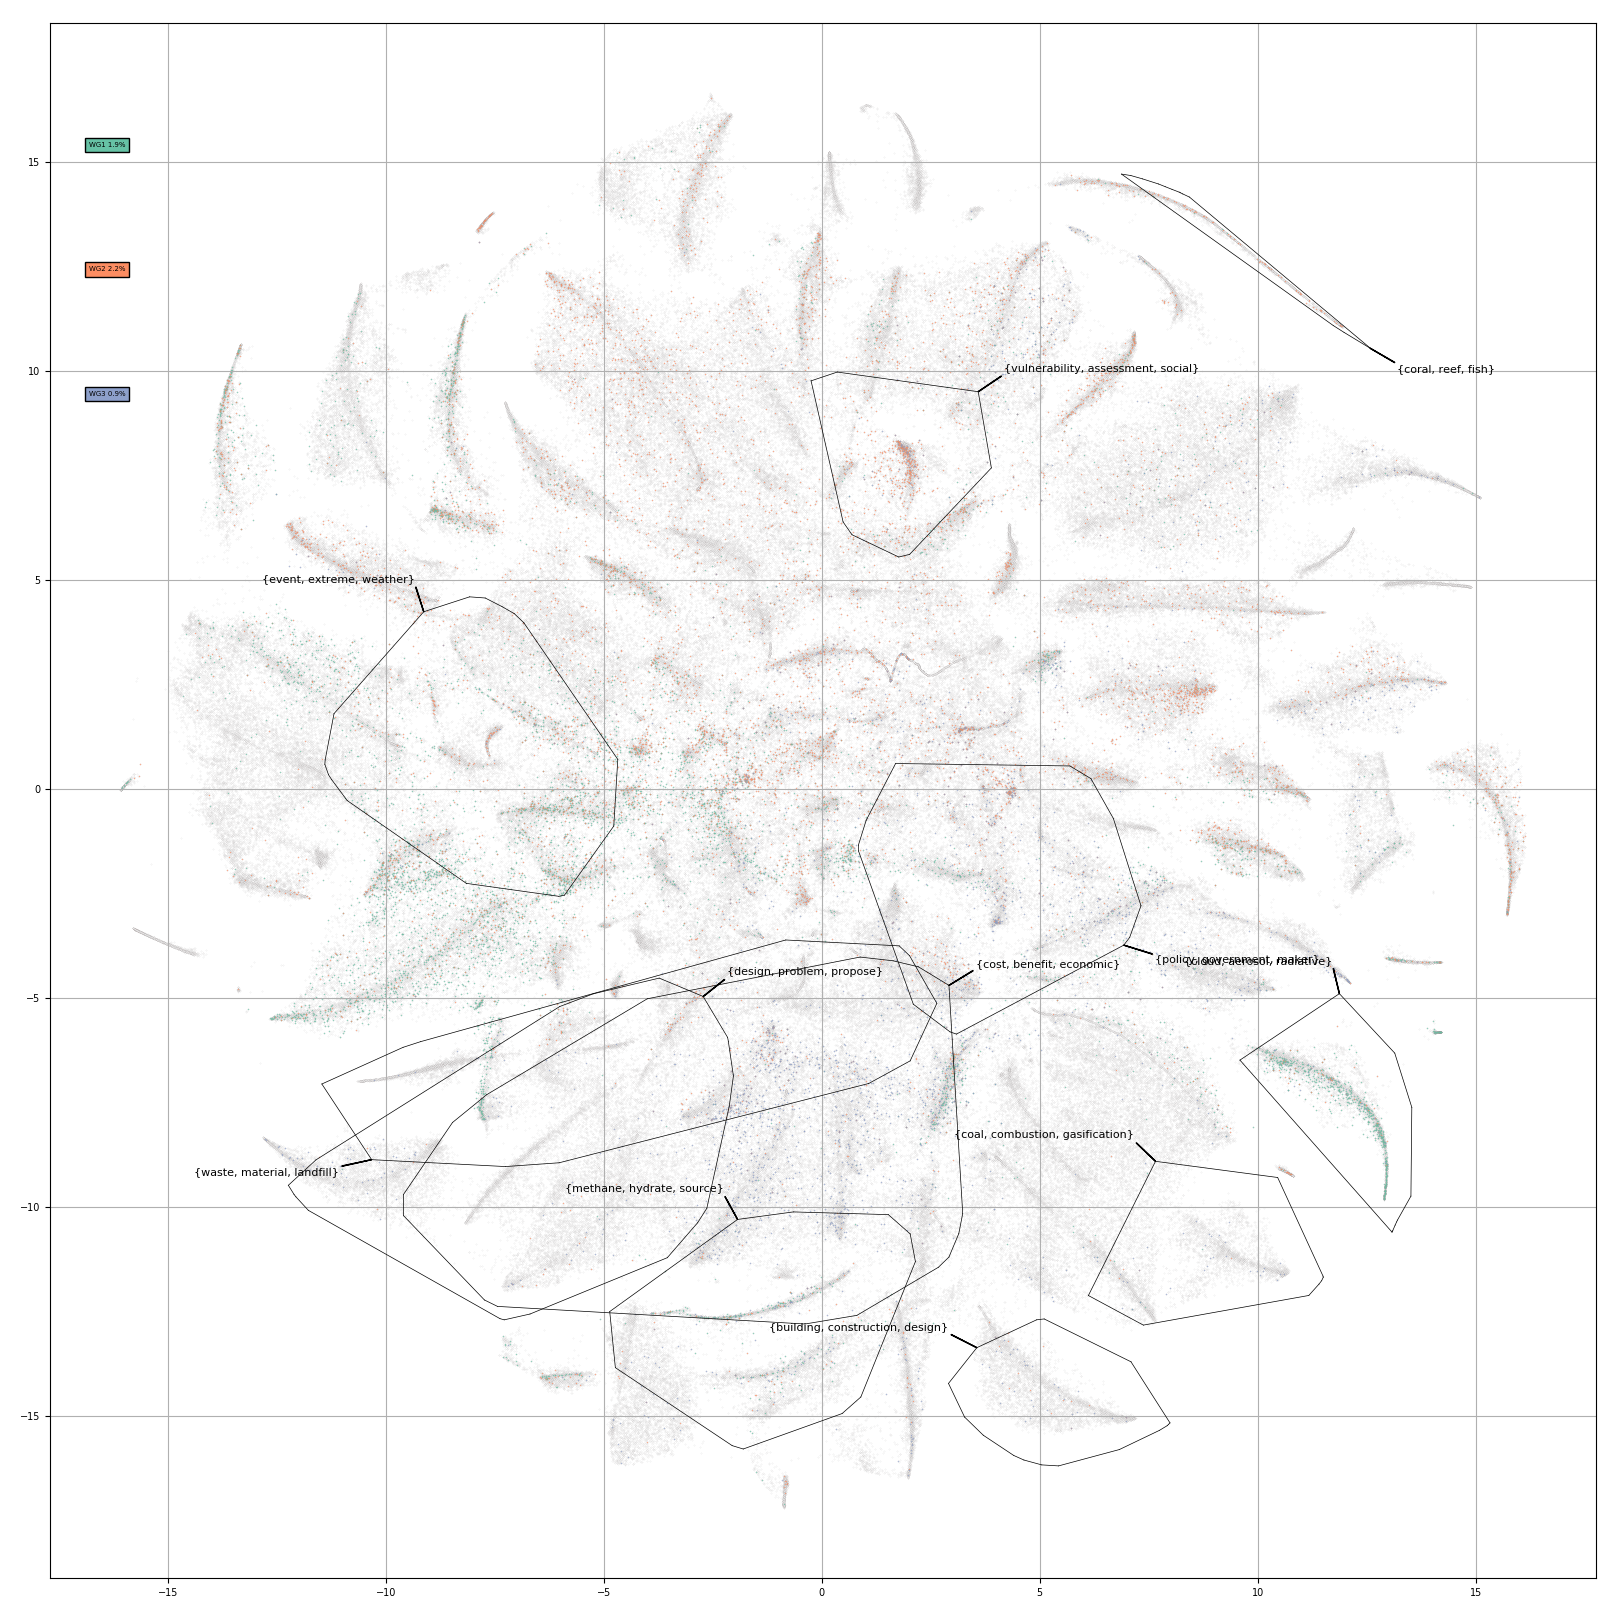
\includegraphics[width=0.8\linewidth]{../tsne_results/plots/run_1429_s_0_p50_interesting_topics_wgs.png}
		}<2->
		\label{map-wgs}
\end{figure}
	\end{column}
	\begin{column}{0.382\linewidth}
		\begin{itemize}
	\item The thematic structure is also reflected in the division of labour between IPCC working groups. Documents cited by each working group appear in discrete parts of the map (which correspond also to the disciplinary structure)


		\end{itemize}
	\end{column}
\end{columns}
\end{frame}

%%%%%%%%%%%%%%%%%%%%%%%%%%%%%%%%%%

\begin{frame}{Newness and representation}
\begin{columns}
	\begin{column}{0.618\linewidth}
\begin{figure}[h!]
	\begin{center}
		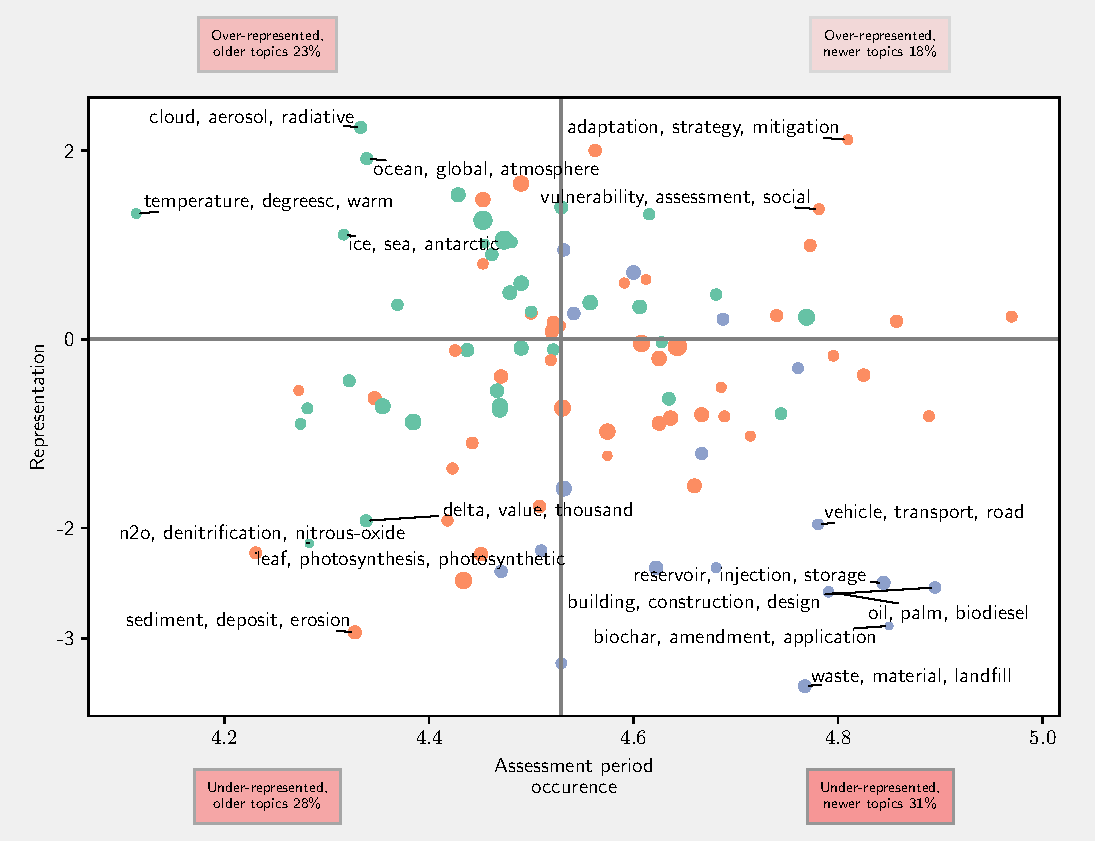
\includegraphics[width=0.85\linewidth]{../plots/ipcc_representation/ipcc_rep_new1429_all.pdf}
		\caption{The IPCC representation and age of the topics. Representation shows the log of the share of topic documents in IPCC citations divided by the share of topic documents among all documents. Assessment period occurence shows the assessment period in which the mean topic document was published}
		\label{ipcc_rep}
	\end{center}
\end{figure}
	\end{column}
	\begin{column}{0.382\linewidth}
		\begin{itemize}
			\item<2-> Those topics that deal with working group III \textit{solutions} issues (materials and recycling, negative emissions, buildings) are in general fast growing and under-represented in IPCC reports
			\item<3-> Some working group III topics (on scenarios, on policies, and on international trade and cross country comparisons) are however over-represented in IPCC reports [see SI]
			\item<4-> Working group I topics are in general older and better represented
			\item<5-> Of the newer topics that are well represented, many are on WG II issues	
			
		\end{itemize}
	\end{column}
\end{columns}
\end{frame}

\section{Conclusions}

\begin{frame}{Conclusions}

\begin{itemize}
	\item<1-> Comparing IPCC citations to wider set of documents sheds new light on imbalances/biases within the IPCC
	\begin{itemize}
		\item Perception of lack of social science knowledge on climate change may be justified, but implications for wider research community, not just IPCC
	\end{itemize}
	\item<2-> Topic modelling enriches our understanding of the content of literature that is emerging, and that is over- or under-represented by the IPCC
	\begin{itemize}
		\item Topics suggest that policymakers' demand for ``solution'' orientated scientific assessments \citep{Kowarsch2017}, may be justified, and possible to achieve with an adjustment of IPCC focus
	\end{itemize}
	\item<3-> The IPCC, not a topic model, is in the best position to decide on what literature to cite
		\begin{itemize}
			\item But, the IPCC can best make these decisions when supported by machines to find out what is out there.
		\end{itemize}
\end{itemize}

\end{frame}

%%%%%%%%%%%%%%%%%%%%%%%%%%%%%%
%% Bib

\begin{frame}{Bibliography}
\small
\bibliography{../Mendeley}
\end{frame}

\begin{frame}{Thanks for your attention}
\begin{columns}
	\begin{column}{0.5\linewidth}
						\begin{figure}
			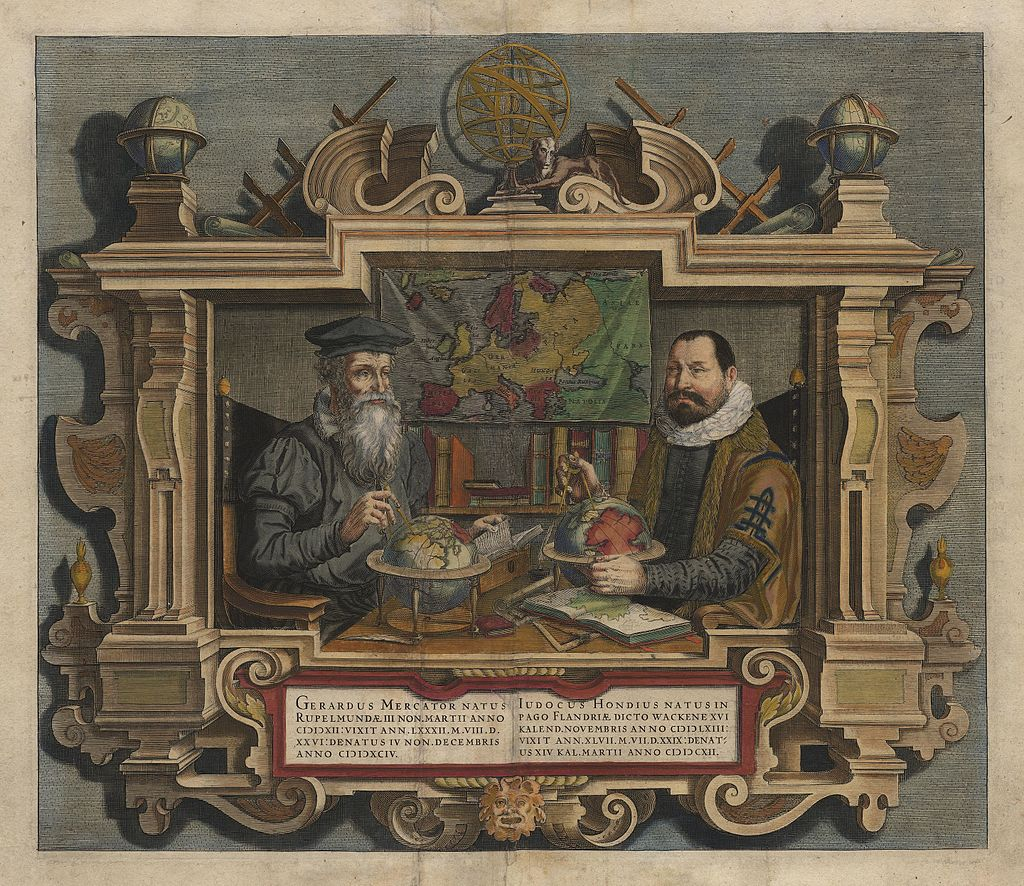
\includegraphics[width=1\linewidth]{../plots/Hondius_Portrait_of_map-makers}
		\end{figure}
	\end{column}
	\begin{column}{0.5\linewidth}
			\begin{figure}
		\begin{center}
			%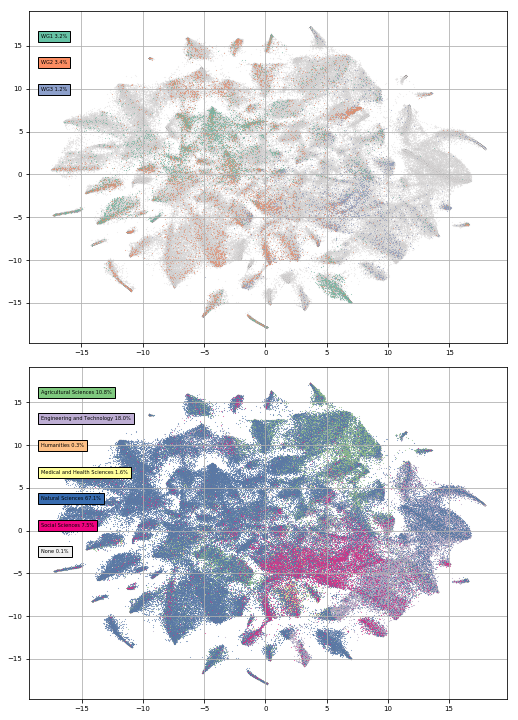
\includegraphics[width=1\linewidth]{tsne_results/plots/run_665_s_0_p200_double.pdf}
			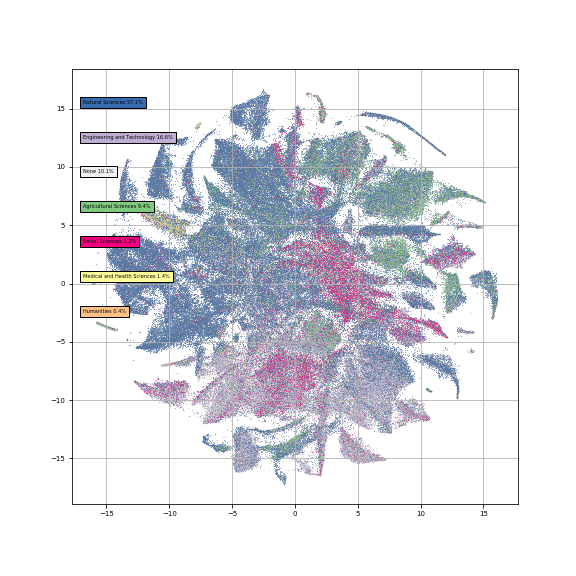
\includegraphics[width=1\linewidth]{../tsne_results/plots/run_1429_s_0_p50_oecds.png}
		\end{center}
	\end{figure}
	\end{column}
\end{columns}
\end{frame}

%%%%%%%%%%%%%%%%%%%%%%%%%%%%%%%%%%

%%%%%%%%%%%%%%%%%%%%%%%%%%%%%%%%%%

\begin{frame}{Doc Topic Example}
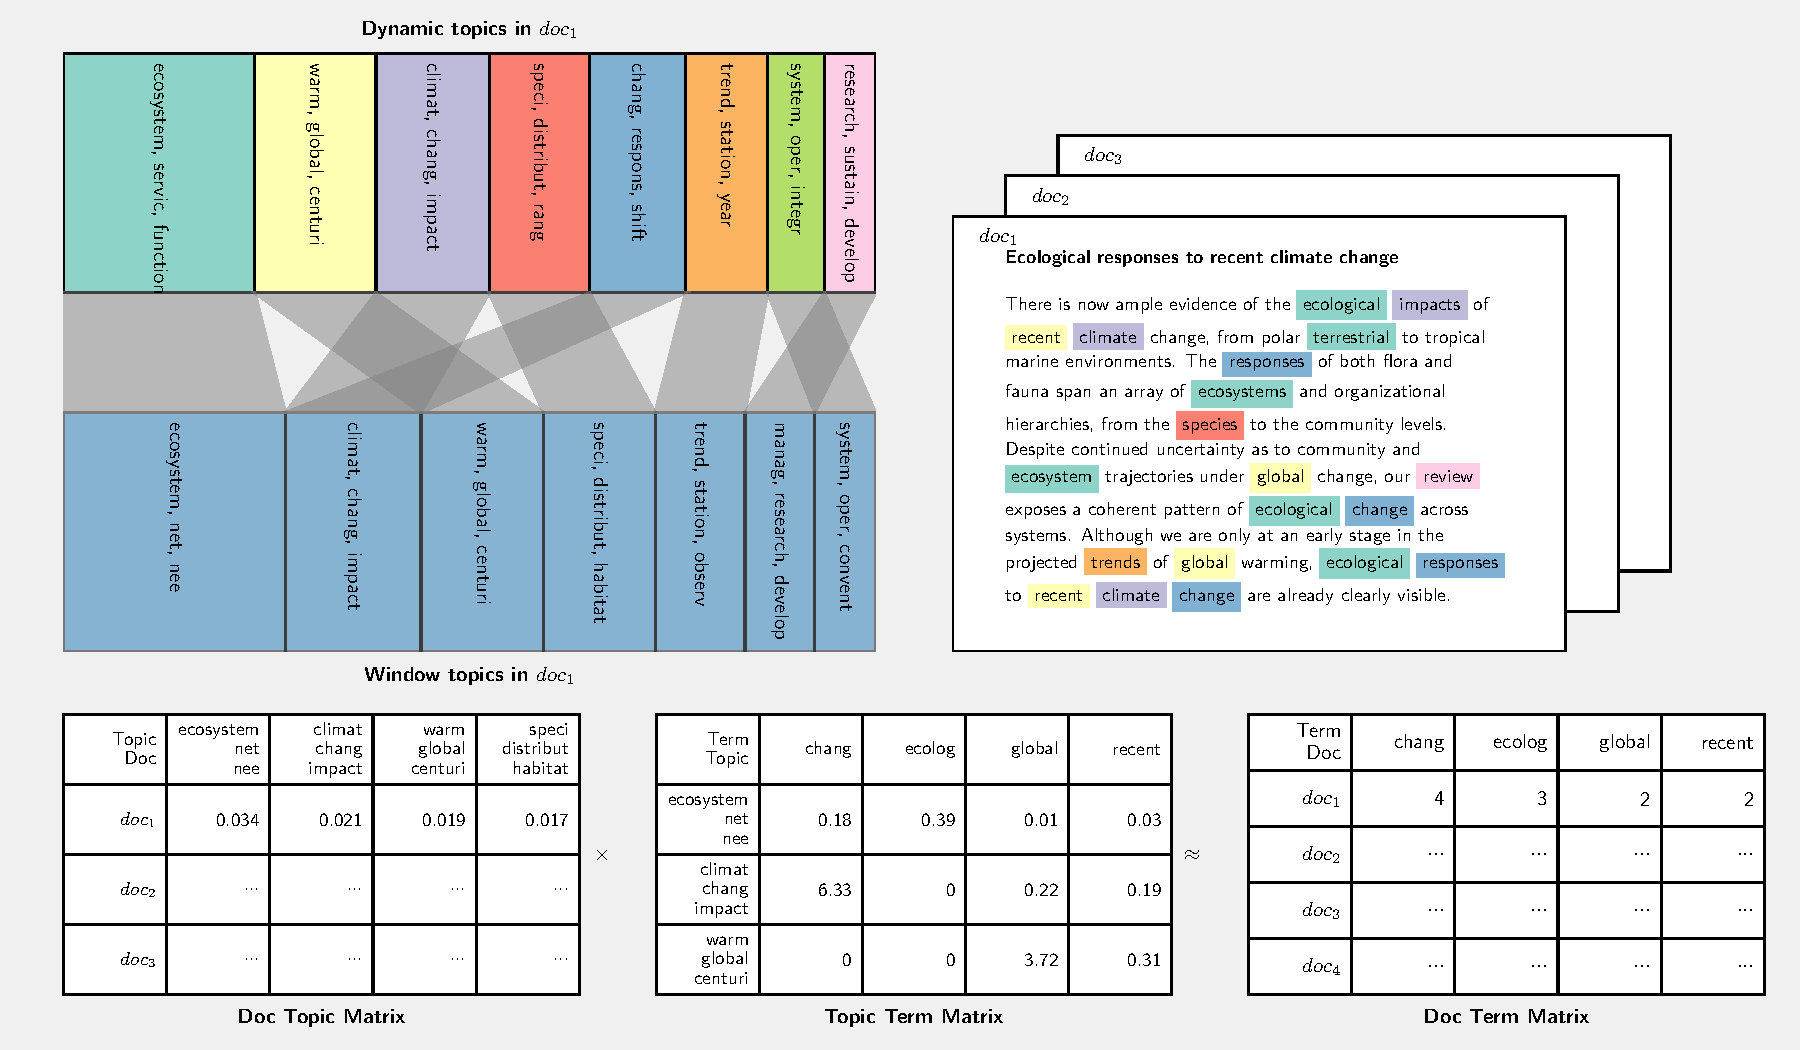
\includegraphics[width=\linewidth]{../plots/single_doc_3_ex.pdf}
\end{frame}

%%%%%%%%%%%%%%%%%%%%%%%%%%%%%%%

\end{document}